\section{Признаки сходимости положительных рядов}

\begin{Def}~\\
	Числовой ряд $\baserow{a_n}$ называется положительным, что эквивалентно
    \[
         \forall n \in \bb{N} \quad a_n \geqslant 0
    \]
\end{Def}

\begin{Th}~\\
	Пусть $\sum\limits_{n = 1}^{+\infty}a_n$ --- положительный ряд, частичные суммы $S_n$ которого ограничены сверху. Тогда ряд $\baserow{a_n} = S$ сходится и его сумма равна 
    \[
        S = \underset{n \geqslant 1}{\sup}(S_n)
    \]
\end{Th}

\begin{Proof}~\\
    Так как ряд положительный, то очевидно что
    \[
        \forall n \geqslant 1 \quad S_{n+1} = S_n + a_n \geqslant S_n
    \]
    Значит последовательность $\{S_n\}$ возрастает.\\
    Также
    \[
        \exists \lim_{n \to +\infty}S_n
    \]
    это эквивалентно последовательности $\{S_n\}$, которая по условию ограничена сверху и её предел равен 
    \[
        S = \underset{n \geq 1}{sup}(S_n)
    \]
\end{Proof}

Ограниченность суммы сверху означает то, что она всегда стремится к некоторому значению, но не превосходит его. Если это мысленно представить, то станет очевиден факт того что ряд с таким свойством частичных сумм будет иметь на бесконечном промежутке конечное значение суммы, так как, например, слагаемые могут уменьшаться и становится очень малыми. Также данный факт был рассмотрен при доказательстве формулы для убывающей геометрической прогрессии (см. предыдущий параграф).

%Короче, если из бесконечного множества частных сумм ряда ни одна не превышает какого-то числа, то ряд точно сходится. Причём схоится к большей из этого бесконечного числа сумм.

\pagebreak

\begin{Th}[Признак сравнения сходимости рядов]~\\
	Пусть $\baserow{a_n}$ и $\baserow{b_n}$ --- два ряда. При этом:
	\begin{enumerate}
		\item $\forall n \geq 1 \quad a_n \geq 0$ (ряд положительный)
        
		\item $\exists n_0 \in \bb{N} \quad \forall n \geqslant n_0 \quad |b_n| \leqslant a_n$
        
		\item Ряд $\baserow{a_n}$ сходится
	\end{enumerate}
	Тогда $\baserow{b_n}$ сходитсsя
\end{Th}

\begin{Proof}~\\
    Ряд $\baserow{a_n}$ сходится то по критерию Коши следует
    \begin{gather*}
       \forall \varepsilon > 0 \quad \exists N \geq n_0 \quad \forall p \in \bb{N} \quad \forall n \geq N \quad |a_{n+1} + \dots + a_{n+p}| < \varepsilon
    \end{gather*}
	Воспользуемся неравенством из условия и распишем его, пользуясь неравентсвом треугольника
    \begin{gather*}
        |b_{n+1} + \dots + b_{n+p}| \leqslant |b_{n+1}| + \dots + |b_{n+p}| \leqslant a_{n+1} + \dots + a_{n+p}  
    \end{gather*}
    Зная, что ряд $a_n$ положительный, получим
    \begin{gather*}
       a_{n+1} + \dots + a_{n+p} = |a_{n+1} + \dots + a_{n+p}| < \varepsilon
    \end{gather*}
    Объединим два неравенства выше и получим следующее неравентсво
    \[
        |b_{n+1} + \dots + b_{n+p}| < \varepsilon
    \]
    По критерию Коши, ряд $\baserow{b_n}$ сходится.
\end{Proof}

\begin{Seq}~\\
    Если
	\[
        \forall n \geq n_0 \quad 0 \leqslant b_n \leqslant a_n 
    \] 
    и ряд $\baserow{b_n}$ расходится, то и $\baserow{a_n}$ тоже расходится
\end{Seq}

\begin{Proof}~\\
	От противного:\\
	Если бы $\baserow{a_n}$ сходился, то по теореме 2 $\baserow{b_n}$ --- сходится. Получаем противоречие
\end{Proof}

\begin{Th}[Признак сравнения рядов в предельной форме]~\\
	Пусть 
    \[
        \forall n \geq 1 \quad a_n \geqslant 0, \quad b_n \geqslant 0 \quad \exists \lim_{n \to +\infty}\frac{a_n}{b_n} = c \neq 0 \quad (c > 0)
    \]
	Тогда если ряд $\baserow{a_n}$ сходится, то ряд $\baserow{b_n}$ сходится, и наоборот.
\end{Th}

\begin{Proof}~
    \begin{enumerate}
        \item[\textcolor{blue}{$\Rightarrow$}] $\baserow{a_n}$ сходится, а также по условию
        \[
            \lim_{n \to +\infty} \frac{a_n}{b_n} = c
        \]
        Пусть $\varepsilon = \frac{c}{2} (\varepsilon > 0)$, тогда 
        \begin{gather*}
             \exists n_0 \in \bb{N} \quad \forall n \geqslant n_0 \quad \left|\frac{a_n}{b_n} - c\right| < \frac{c}{2} 
        \end{gather*}
        Раскроем знак модуля в неравентстве, получим
        \begin{gather*}
            \frac{c}{2} < \frac{a_n}{b_n} < \frac{3\,c}{2}\\
            \forall n \geqslant n_0 \quad 0 < b_n < \frac{2}{c}\,a_n
        \end{gather*}
        Ряд $\baserow{a_n}$ сходится, тогда по теореме 2 ряд $\baserow{b_n}$ сходится.\\
        
        \item[\textcolor{blue}{$\Leftarrow$}] Ряд $\baserow{b_n}$ сходится, тогда аналогично получаем
        \[
            \forall n \geq n_0 \quad a_n < \frac{3}{2}\,c\,b_n
        \]
        По теореме 2 $\baserow{a_n}$ сходится.
    \end{enumerate}
\end{Proof}

\begin{Note}~\\
    Теорема спрвадлива и для расходящихся рядов.\\
    Если один из рядов расходится, то и другой расходится.
\end{Note}

%Аналогичная штука работает для расходящихся рядов:\\
%Если предел отношения элементов ряда на бесконечности равен ненулевой константе и один из рядов расходящийся, то и второй тоже обязательно расходится

\textcolor{red}{не разобран}
\begin{Example}~
	\begin{enumerate}
		\item ряд $\baserow{\ln(1+\frac{1}{n})}$ расходится $(1)$ \\
			$\ln(1+t) \sim t (t \to 0) \Rightarrow [t=\frac{1}{n}] \Rightarrow \ln(1+\frac{1}{n}) \sim \frac{1}{n} (n \to +\infty) \Rightarrow\\
			\Rightarrow \lim\limits_{n \to +\infty} \frac{\ln(1+\frac{1}{n})}{\frac{1}{n}} = 1 \neq 0$ \\
			Теперь, учитывая, что у нас есть ненулевой предел отношения элементов двух рядов, один из которых расходящийся, можно говорить, что расходится и второй, т.е. ряд $\baserow{\frac{1}{n}}$ расходится
		\item ряд $\baserow{\frac{1}{n(n+1)}} = 1$ сходится. $(S_n = 1 - \frac{1}{n+1}) \Rightarrow$ ряд $\baserow{\frac{1}{n^2}}$ сходится, т.к. $\lim\limits_{n \to +\infty}\frac{\frac{1}{n(n+1)}}{\frac{1}{n^2}} = 1$
	\end{enumerate}
\end{Example}

\begin{Th}[Признак Даламбера]~\\
	Пусть $\forall n \geq 1 \: a_n > 0$ и
	\begin{enumerate}
		\item ряд $\baserow{a_n}$ сходится если
        \[
            \exists q < 1 \quad \forall n \geqslant n_0 \quad \frac{a_{n+1}}{a_n} \leqslant q \leqslant 1
        \]
		
        \item ряд $\baserow{a_n}$ расходится если 
        \[
            \forall n \geqslant n_0 \quad \frac{a_{n+1}}{a_n} \geqslant 1
        \] 
	\end{enumerate}
\end{Th}

\begin{Proof}~
	\begin{enumerate}
		\item Дано 
        \[
            \frac{a_{n+1}}{a_n} \leqslant q < 1 \qquad (\forall n \geqslant n_0)
        \]
        Из этого можно вывести следующую цепочку
        \[
            a_n \leqslant a_{n-1}\,q \leqslant a_{n-2}\,q^2 \leqslant \dots \leqslant a_{n_0}\,q^{n-n_0}
        \]
        Рассмотрим цепочку как ряд и найдём его сумму
        \[
            \sum_{n=n_0}^{+\infty}a_{n_0}\,q^{n-n_0} = a_{n_0}\,\sum_{k = 0}^{+\infty}q^k
        \]
        Так как $q < 1$, следовательно перед нами убывающая геометрическая прогрессия. По формуле сумма равна
        \[
		  a_{n_0}\sum_{k = 0}^{+\infty}q^k = \frac{a_{n_0}}{1-q}
        \]
        Значит частичные суммы ряда ограниченны,  следовательно по теореме 1, ряд $\baserow{a_n}$ сходится.
        
		\item Дано 
        \[
            \frac{a_{n+1}}{a_n} \geqslant 1 \qquad (\forall n \geqslant n_0)
        \]
        Из этого следует
        \begin{gather*}
            a_n \geqslant a_{n-1} \geqslant \dots \geqslant a_{n_0} > 0\\
            a_n \geq a_{n_0} > 0 \qquad (n \to +\infty)
        \end{gather*}
        если бы $a_n \to 0$ (необходимое условие сходимости ряда), тогда по принципу сжатой переменной $a_{n_0} = 0$, но это не так, есть противоречие. Значит $a_n \nrightarrow 0 (n \to +\infty)$ и ряд расходится.
	\end{enumerate}
\end{Proof}

\begin{Th} [Признак Даламбера в предельной форме]~\\
	Пусть 
    \[
        \forall n \geqslant 1 \quad a_n > 0 \quad \exists \lim_{n \to +\infty}\frac{a_{n+1}}{a_n} = q
    \]
    тогда ряд $\baserow{a_n}$:
	\begin{enumerate}
		\item сходится, если $q < 1$
		\item расходится, если $q > 1$
		\item при $q = 1$ может сходиться или расходиться
	\end{enumerate}
\end{Th}

\begin{Proof}~
	\begin{enumerate}
		\item Дано
        \[
            \lim_{n \to +\infty}\frac{a_{n+1}}{a_n} = q, \qquad q < 1
        \]
        Возьмём
        \[
            \varepsilon = \frac{1-q}{2} > 0
        \]
        $\varepsilon > 0$ так как по условию $q < 1$.\\
        Из определения предела по Коши получаем
        \[
            \exists n_0 \in \bb{N} \quad \forall n \geqslant n_0 \quad \left|\frac{a_{n+1}}{a_n}-q\right| < \frac{1-q}{2}
        \]
        Раскроем знак модуля, а также воспользуемся $q < 1$, и в итоге получим
        \begin{gather*}
            q-\frac{1-q}{2} < \frac{a_{n+1}}{a_n} < q+\frac{1-q}{2} = \frac{q+1}{2} = q^{\ast} < \frac{1 + 1}{2} = 1 \\
            \forall n \geqslant n_0 \qquad \frac{a_{n+1}}{a_n} < q^{\ast} < 1 
        \end{gather*}
        Таким образом, по теореме 4 следует, что $\baserow{a_n}$ сходится
		
        \item Дано
        \[
            \lim_{n \to +\infty}\frac{a_{n+1}}{a_n} = q, \qquad q>1
        \]
        Аналогично выбираем занчение $\varepsilon$
        \[
            \varepsilon = \frac{q-1}{2} > 0
        \]
        Далее всё аналогично
        \begin{gather*}
            \exists n_0 \in \bb{N} \quad \forall n \geq n_0 \quad \left|\frac{a_{n+1}}{a_n} - q\right| < \frac{q-1}{2}\\ 
            q-\frac{q-1}{2} < \frac{a_{n+1}}{a_n} < q+\frac{q-1}{2}\\
            1 = \frac{1 + 1}{2} < q^{\ast} = \frac{q+1}{2} < \frac{a_{n+1}}{a_n}\\
            \forall n \geqslant n_0 \qquad 1 < q^{\ast} < \frac{a_{n+1}}{a_n}
        \end{gather*}
		Аналогично по теореме 4 получаем, что $\baserow{a_n}$ расходится
		
        \item Дано 
        \[
            \lim_{n \to +\infty}\frac{a_{n+1}}{a_n} = q \qquad q = 1
        \]
		Для доказательства достаточно привести примеры сходящегося и расходящегося ряда для $q = 1$:
		\begin{itemize}
			\item Пример расходящегося ряда
            \[
                \baserow{\frac{1}{n}} \qquad \frac{a_{n+1}}{a_n} = \frac{n}{n+1} \to 1 \quad (n \to +\infty)
            \]
			\item Пример сходящегося ряда 
            \[
                \baserow{\frac{1}{n^2}} \qquad \frac{a_{n+1}}{a_n} = \frac{n^2}{(n+1)^2} \to 1 \quad (n \to +\infty)
            \]
		\end{itemize}
	    Таким образом, при $q=1$ существует неопределённость.
	\end{enumerate}
\end{Proof}

\begin{Th}[Радикальный метод Коши]~\\
	Пусть 
    \[
        \forall n \geqslant 1 \quad a_n > 0 \quad \exists \lim_{n \to +\infty}\sqrt[n]{a_n} = l, \quad l \in \bb{R}
    \] 
    Тогда ряд $\baserow{a_n}$:
	\begin{enumerate}
		\item сходится при $l < 1$  
		\item расходится при $l > 1$
		\item может сходиться или расходиться при $l = 1$
	\end{enumerate}
\end{Th}

\begin{Proof}~
	\begin{enumerate}
		\item Дано $l < 1$, тогда $0 \leqslant l < 1$\\
        Возьмём значение $\varepsilon > 0$ и тогда по определению предела по Коши получим
        \[
            \varepsilon = \frac{1-l}{2} \quad \exists n_0 \in \bb{N} \quad \forall n \geqslant n_0 \quad |\sqrt[n]{a_n} - l| < \frac{1-l}{2}
        \]
        Раскроем модуль
        \begin{gather*}
            \sqrt[n]{a_n} < \frac{l+1}{2} = l^{\ast} < 1\\
            a_n < (l^{\ast})^n \quad (n \geqslant n_0) \quad l^{\ast} \in [0;1]
        \end{gather*}
		ряд $\sum\limits_{n = n_0}^{+\infty}(l^{\ast})^n$ сходится, т.к. это убывающая геометрическая прогрессия, следовательно по теореме 2 ряд $\baserow{a_n}$ сходится.
        
		\item Дано $l > 1$. Доказательство аналогино
        \begin{gather*}
            \varepsilon = \frac{l-1}{2} \quad \exists n_0 \in \bb{N} \quad \forall n \geq n_0 \quad \left|\sqrt[n]{a_n} - l\right| < \frac{l-1}{2}\\
            1 < l^{\ast} = \frac{l+1}{2} = l - \frac{l-1}{2} < \sqrt[n]{a_n} \quad (n \geqslant n_0)\\
            \forall n \geqslant n_0 \quad a_n > 1 \quad a_n \nrightarrow 0 (n \to +\infty)
        \end{gather*}
        Таким образом, ряд $\baserow{a_n}$ расходится
		
        \item Для доказательства достаточно привести примеры сходящегося и расходящегося ряда
		\begin{itemize}
			\item ряд $\baserow{1}$ расходится
            \[
                a_n = 1, \quad \sqrt[n]{a_n} = 1, \quad \sqrt[n]{a_n} \to 1 \quad (n \to +\infty) \quad \Rightarrow \quad l=1
            \]
			
            \item ряд $\baserow{\frac{1}{n^2}}$ сходится (т.к. гармонический ряд) 
            \[
                \sqrt[n]{a_n} = (\frac{1}{n^2})^{\frac{1}{n}} = e^{-2\frac{\ln n}{n}} \to 1 \quad (n \to +\infty) \quad \Rightarrow \quad l = 1
            \]
		\end{itemize}
	\end{enumerate}
\end{Proof}

\begin{Th}[Интегральный признак Коши]~\\
	Пусть функция $f(x)$ удовлетворяет условиям:
	\begin{enumerate}
		\item $f(x) \in C_{[1;+\infty)}$
		\item $f(x)$ убывает на $[1;+\infty)$
		\item $\forall x \in [1; + \infty) \quad f(x) > 0$
	\end{enumerate}
	Тогда ряд $\baserow{f(n)}$ сходится $\Leftrightarrow$ несобственный интеграл $\int\limits_{1}^{+\infty}f(x)\,dx$ сходится
\end{Th}

\pagebreak

\begin{Proof}~\\
    \begin{figure}[bh]
       \noindent\centering{
            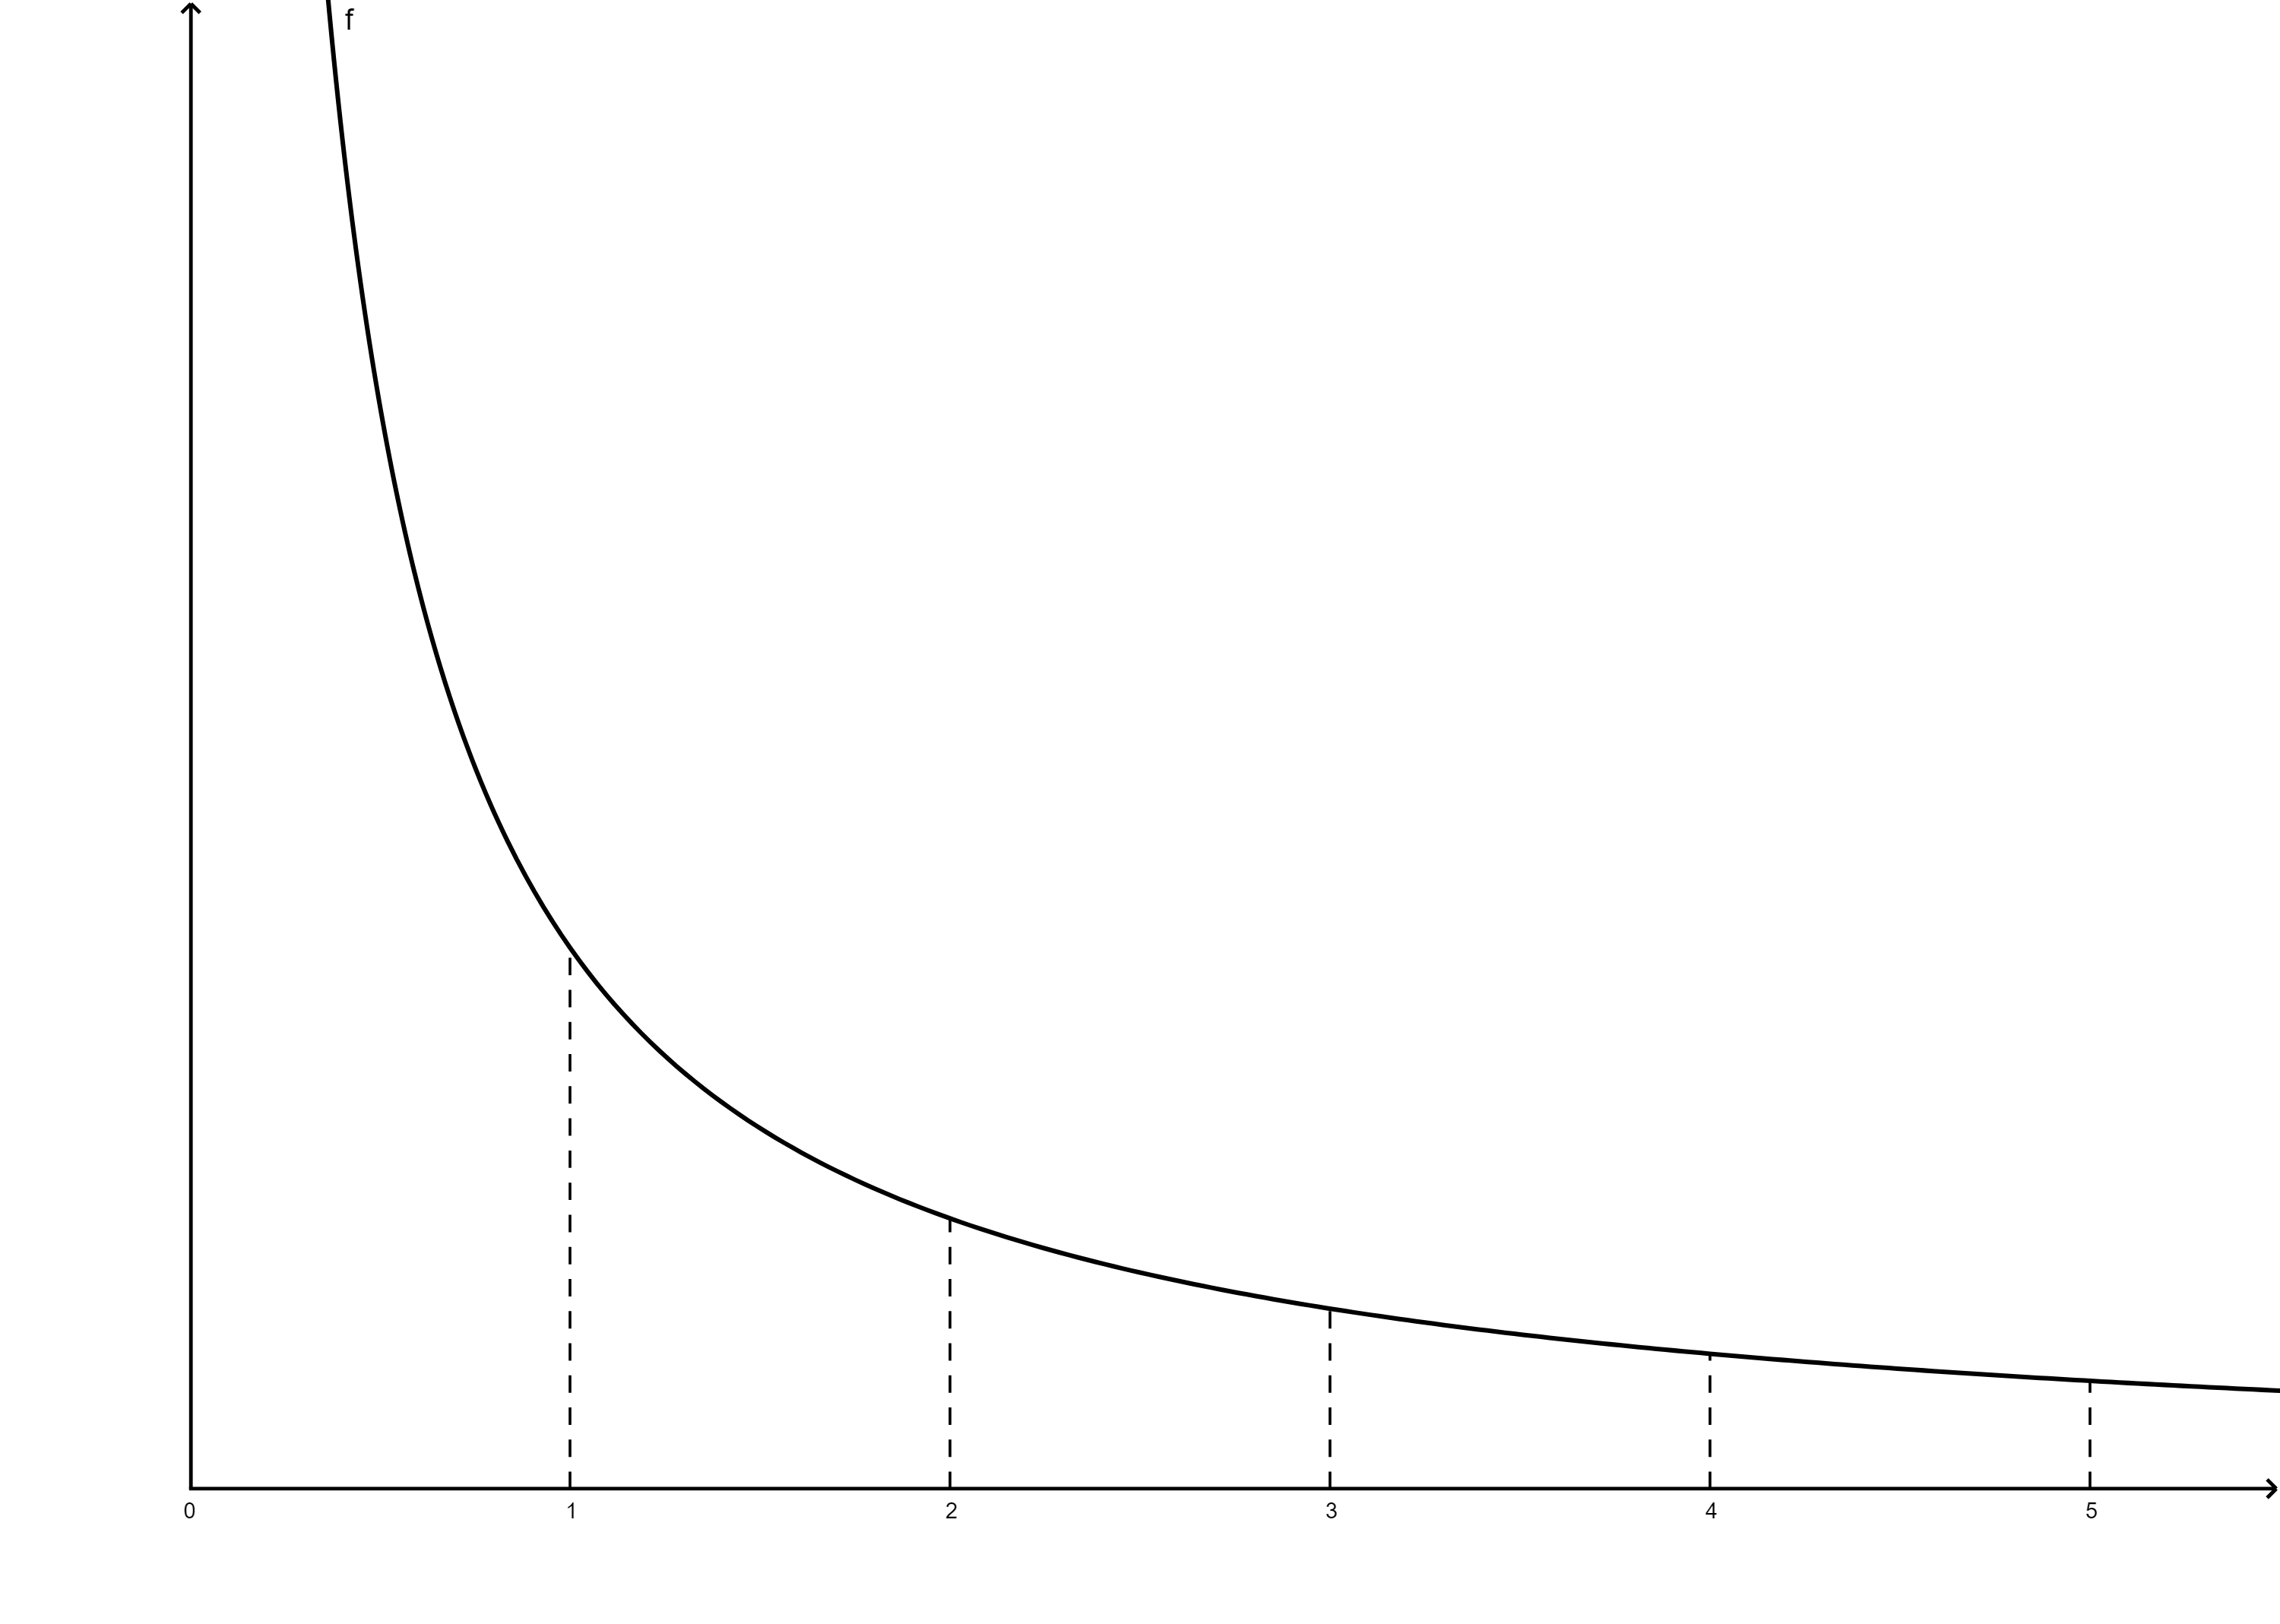
\includegraphics[width=55mm]{pictures/3_2_1.png}
            \caption{}
       }
    \end{figure}
    Из условия
    \[
        x \in [k; k+1], \quad f(k+1) < f(x) < f(k) \quad (k=1,2,\dots)
    \]
    Следовательно
    \begin{align*}
        f(k+1) \leqslant &\int_{k}^{k+1}f(x)\,dx \leqslant f(k)\\
        \sum_{k=1}^{n}f(k+1) \leqslant &\int_{1}^{n+1}f(x)\,dx \leqslant \sum_{k=1}^{n}f(k) = S_n\\ 
        S_{n+1} - f(1) \leqslant &\int_{1}^{n+1}f(x)\,dx \leqslant S_n
    \end{align*}
    \begin{enumerate}
        \item[\textcolor{blue}{$\Rightarrow$}] Дано $\baserow{f(n)}$ сходится, следовательно по  теореме 1 $S_n \leqslant S$.\\
        По аксиоме Архимеда
        \[
            \forall t \in \bb{R} \quad t > 1 \quad \exists n \in \bb{N} \quad t<n+1
        \]
        \textcolor{red}{ниже не понятно}
        $F(t) = \int_{1}^{t}f(x)\,dx = \int_{1}^{n+1}f(x)\,dx \leqslant S_n \leqslant S$\\
        $F(t) \nearrow$ т.к. $F'=f(x) \Rightarrow \exists \lim\limits_{t \to +\infty} = F \leq S \Rightarrow \int\limits_{1}^{+\infty}f(x)\,dx$ сходится\\
        
        \item[\textcolor{blue}{$\Leftarrow$}] Дано	$\int_{1}^{+\infty}f(x)\,dx = F$ сходится, тогда
        \[
            S_n \leqslant f(1) + \int_{1}^{n+1}f(x)\,dx \leqslant f(1) + F
        \] 
        Очевидно что по теореме 1 ряд $\baserow{f(n)}$ сходится.
    \end{enumerate}
\end{Proof}